\documentclass[unicode]{beamer}
\usepackage{lmodern}
\usetheme{Dresden}
\usecolortheme{beaver}
\usefonttheme{professionalfonts}
%\usefonttheme{structurebold}
\usepackage{times}
\usepackage{tikz}
\usepackage{array}
\usepackage{amsmath}
\usepackage{verbatim}
%\usepackage{kotex}
\usepackage{multirow}
\usepackage{epstopdf}
\usepackage{color}
\usetikzlibrary{arrows,shapes}

\title{\bf Dirichlet Process}

\author{\bf DaeYoung Lim and SeoYoon Cho}
\date{2016.05.16 (Mon)}

\newcommand{\frameofframes}{/}
\newcommand{\setframeofframes}[1]{\renewcommand{\frameofframes}{#1}}

\setframeofframes{of}
\makeatletter
\setbeamertemplate{footline}
  {%
    \begin{beamercolorbox}[colsep=1.5pt]{upper separation line foot}
    \end{beamercolorbox}
    %\begin{beamercolorbox}[ht=2.5ex,dp=1.125ex,%
    %  leftskip=.3cm,rightskip=.3cm plus1fil]{author in head/foot}%
    %  \leavevmode{\usebeamerfont{author in head/foot}\insertshortauthor}%
    %  \hfill%
    %  {\usebeamerfont{institute in head/foot}\usebeamercolor[fg]{institute in head/foot}\insertshortinstitute}%
    %\end{beamercolorbox}%
    \begin{beamercolorbox}[ht=2.5ex,dp=1.125ex,%
      leftskip=.3cm,rightskip=.3cm plus1fil]{title in head/foot}%
      {\usebeamerfont{title in head/foot}\insertshorttitle}%
      \hfill%
      {\usebeamerfont{frame number}\usebeamercolor[fg]{frame number}\insertframenumber~\frameofframes~\inserttotalframenumber}
    \end{beamercolorbox}%
    \begin{beamercolorbox}[colsep=1.5pt]{lower separation line foot}
    \end{beamercolorbox}
  }
\makeatother

\begin{document}
\maketitle

\frame{\frametitle{Contents}
\begin{itemize}
  \item Dirichlet Distribution
  \item Definition of Dirichlet Process
  \item Properties of DP
  \item Dirichlet Process Mixtures
\end{itemize}}

\section{Dirichlet Distribution}
\subsection{}

\frame{\frametitle{Dirichlet-Multinomial Model}
\begin{itemize}
  \item[-] Prior and Model
  \begin{eqnarray*}
  Y_i |p &\stackrel{ind}{\sim}&\text{Multinomial}(p),\ \ \ \ \ i=1,\cdots,n\\
  p=(p_1 ,\cdots,p_k )&\sim&\text{Dirichlet}(\alpha_1 ,\cdots,\alpha_k )\\
  \pi(p)&=& \frac{\Gamma(\sum \alpha_i )}{\prod_{i=1}^k \Gamma(\alpha_i )}\prod_{i=1}^k p_i^{\alpha_i -1}
  \end{eqnarray*}
  \item[-] Posterior
  $$\text{Dirichlet}(\alpha_1 +\sum I(Y_i =1),\cdots,\alpha_k +\sum I(Y_i =k))$$
  \item[-] Prior \textbf{has full support} and is \textbf{conjugate}, thus leading to an easy update
\end{itemize}}


\frame{\frametitle{DD to DP}
\begin{itemize}
  \item Dirichlet Distribution
  $$G \sim \text{Dir}(\alpha),\ \ \theta_i |G \sim G$$
  \begin{itemize}
    \item[-] For any measurable set $A$, partition $\mathbf{R}$ into $A$ and $A^c$
    \item[-] Dirichlet-Multinomial (Beta-Binomial) model on $A$ and $A^c$
    $$P(\theta_i \in A)=\frac{\alpha(A)}{\alpha(\mathbf{R})}$$
  \end{itemize}
  \item Dirichlet Process
  $$G \sim \text{DP}(MG_0 ),\ \ \theta_i | G \sim G$$
  \begin{itemize}
    \item[-] Baseline probability distribution $G_0$, mass(precision) parameter $M$, $MG_0 $: base measure of DP
    %\item[-] Posterior
    %  $$\Rightarrow G| \theta_1 ,\cdots,\theta_n \sim \text{DP}\left(M+n,\frac{MG_0 +\sum \delta_{\theta_i}}{M+n}\right)$$
  \end{itemize}
\end{itemize}}

\section{Definition}
\subsection{}

\frame{\frametitle{Ferguson (1973)}
\begin{itemize}
  \item Probability Space : $(\Theta,A,G)$
  \item \textbf{arbitrary} partition $\{A_1 ,\cdots,A_k \}$ of $\Theta$
  \item $G \sim DP(M,G_0 )$ if 
  $$(G(A_1 ),\cdots,G(A_k ))\sim DP(MG_0 (A_1 ),\cdots,MG_0 (A_k ))$$
  \item well-defined infinite dimensional model $p(G)$ because of \textbf{Kolmogorov's consistency conditions} \\({\footnotesize guarantees suitably consistent collection of finite-dimensional distributions define a stochastic process.})
\end{itemize}}

\frame{\frametitle{Kolmogorov's Consistency Conditions}
\begin{itemize}
  \item {\footnotesize Let $T$: interval, $n\in \mathbf{N}$. Then for each $k\in \mathbf{N}$ and finite sequence of times $t_1 ,\cdots,t_k \in T$, let $v_{t_1 \cdots t_k }$ be a probability measure on $(\mathbf{R}^n )^k$ }
\end{itemize}
  \begin{enumerate}
    \item $\forall$ permutations $\pi$ of $\{1,\cdots,k\}$, measurable sets $F_i \subseteq \mathbf{R}^n$,
    $$\mathbf{v_{t_{\pi(1)}\cdots t_{\pi(k)}}(F_{\pi(1)}\times\cdots\times F_{\pi(k)})=v_{t_1 \cdots t_k}(F_1 \times\cdots\times F_k )}$$
    \item For $\forall$ measurable sets $F_i \subseteq \mathbf{R}^n , m\in \mathbf{N},$ 
    $$\textstyle v_{t_1 \cdots t_k}(F_1 \times\cdots\times F_k )=v_{t_1 \cdots t_k t_{k+1} \cdots t_{k+m}}(F_1 \times\cdots\times F_k \times \mathbf{R}^n \times\cdots\times \mathbf{R}^n )$$
  \end{enumerate}
  \begin{itemize}
  \item When the two conditions satisfied, $\exists$ a probability space $(\Omega,F,P)$ and a stochastic process $X: T\times\Omega \rightarrow \mathbf{R}^n $ s.t. $$v_{t_1 \cdots t_k}(F_1 \times\cdots\times F_k )=P(X_{t_1}\in F_1 ,\cdots,X_{t_k}\in F_k )$$ for all $t_i \in T,\ k\in\mathbf{N}$, and measurable sets $F_i \subseteq \mathbf{R}^n$
  \item $X$ has $v_{t_1 \cdots t_k}$ as its finite-dimensional distribution relative to times $t_1 ,\cdots,t_k $
\end{itemize}}

\frame{\frametitle{Sethuraman (1994)}
\begin{itemize}
\item Stick-Breaking Construction
\begin{itemize}
  \item[-] $\delta_{\theta}(\cdot)$: point mass at $\theta$
  \item[-] if $(\tilde{\theta}_h )\stackrel{iid}{\sim}G_0$ 
  \item[-] $v_h \stackrel{iid}{\sim} \text{Beta}(1,M)$
  \item[-] $w_h =v_h \prod_{k<h}\{1-v_k \}$ 
$$G(\cdot)=\sum_{h=1}^{\infty}w_h \delta_{\tilde{\theta}_h}(\cdot)\ \sim DP(M,G_0 )\ \text{prior}$$
\end{itemize}
\end{itemize}}

\frame{\frametitle{Simulation}
\begin{itemize}
  \item[-] $G_0 = \text{Unif}(0,1)$, 1000 samples from $G(\cdot)$
\end{itemize}
\begin{figure}
  \centering
    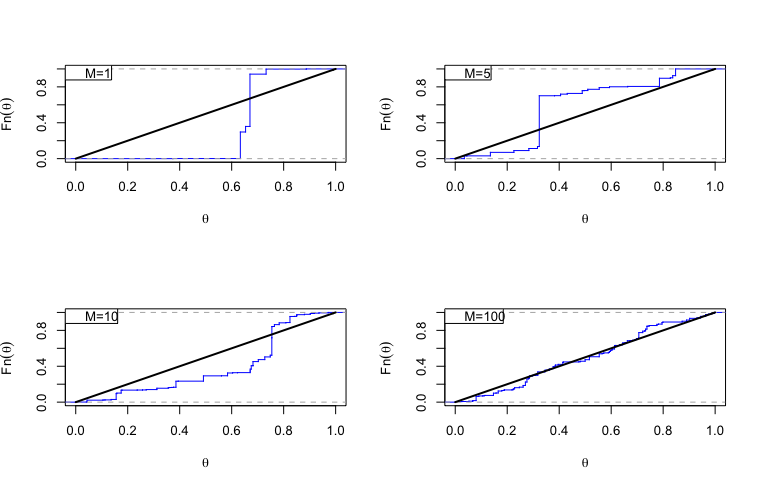
\includegraphics[width=0.8\textwidth]{./SBunif.png}
  %\caption{\footnotesize gray: model (1) , black: model (2) , dashed line: observed value}
\end{figure}}

\frame{\frametitle{Simulation}
\begin{itemize}
  \item[-] $G_0 = \text{N}(0,1)$, 1000 samples from $G(\cdot)$
\end{itemize}
\begin{figure}
  \centering
    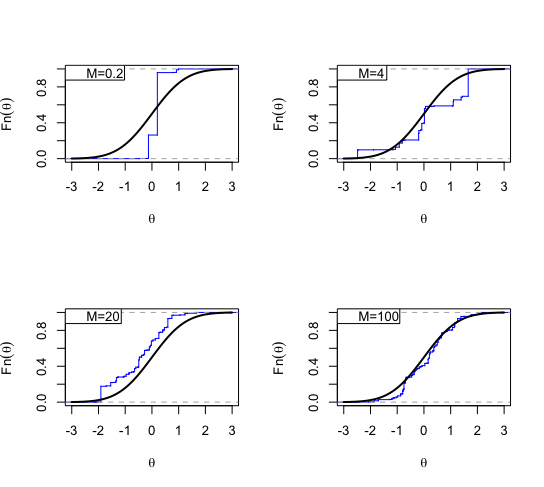
\includegraphics[width=0.65\textwidth]{./SBnorm_M.png}
  %\caption{\footnotesize gray: model (1) , black: model (2) , dashed line: observed value}
\end{figure}}

%\frame{\frametitle{Simulation}
%\begin{itemize}
%  \item[-] $G_0 = \text{N}(0,1)$, $M=5$, 1000 samples from $G(\cdot)$
%\end{itemize}
%\begin{figure}
%  \centering
%    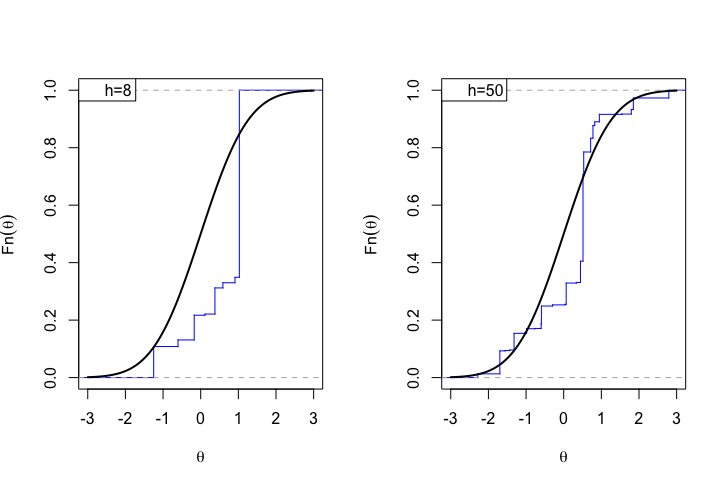
\includegraphics[width=0.8\textwidth]{./SBnorm_h.png}
%  %\caption{\footnotesize gray: model (1) , black: model (2) , dashed line: observed value}
%\end{figure}}

\frame{\frametitle{Simulation Interpretation}
\begin{itemize}
  \item[-] $M\uparrow$ : reduce the variability
  \item[-] $M\downarrow$ : small number of weights concentrate most of the probability mass
\end{itemize}}

\frame{\frametitle{Predictive Probability Function}
\begin{itemize}
  \item $\theta_i |G \stackrel{iid}{\sim}G$ where $G\sim DP(M,G_0 )$.
  \item $k_n$: number of unique values among $\{\theta_1 ,\cdots,\theta_n \}$ 
  \item $\{\theta_1^* ,\cdots,\theta_{k_n}^* \}$ be these unique values
  \item $n_{n_j}$: number of draws among $\{\theta_1 ,\cdots,\theta_n \}$ that are equal to $\theta_j^*$
\end{itemize}
$$p(\theta_{n+1}|\theta_n ,\cdots,\theta_1 )\propto \sum_{j=1}^{k_n}n_{n_j} \delta_{\theta_j^*}+MG_0$$}

\frame{\frametitle{Blackwell and MacQueen (1973)}
  $$p(\theta_{n+1}|\theta_n ,\cdots,\theta_1 )\propto \sum_{j=1}^{k_n}n_{n_j} \delta_{\theta_j^*}+MG_0$$
  \begin{itemize}
    \item[-] new $\theta_i = \theta_j^*$ with probability $\propto n_{n_j}$ 
    \item[ ] or
    \item[-] new $\theta_i$ sampled from $G_0$ with probability $\propto M$.
    \item[-] After integrating $G$, observations are \textbf{exchangeable}, have identical marginal distribution $G_0$ but are not independent.
\end{itemize}}

\frame{\frametitle{Polya Urn (Chinese Restaurant Process)}
\begin{itemize}
  \item Urn has initially \textbf{$M$ black} and \textbf{one colored} ball (color is randomly selected according to $G_0$)
  \item If a \textbf{colored} ball is drawn, return it along with another ball of the \textbf{same color} to the urn
  \item If a \textbf{black} ball is drawn, return it along with a ball of a \textbf{new color} randomly selected according to $G_0$
\end{itemize}}

\frame{\frametitle{Simulation}
\begin{itemize}
  \item[-] $G_0 = \text{Unif}(0,1)$, $M=5$, 10 predictive samples
\end{itemize}
\begin{figure}
  \centering
    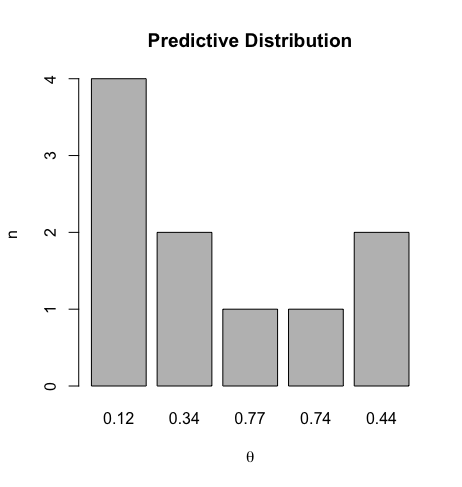
\includegraphics[width=0.55\textwidth]{./crp.png}
  %\caption{\footnotesize gray: model (1) , black: model (2) , dashed line: observed value}
\end{figure}}

\frame{\frametitle{Normalized Random Measure with Independent Increments (NRMI)}
\begin{itemize}
  \item Dirichlet from Gamma
  \begin{eqnarray*}
    y_1 ,\cdots,y_k &\stackrel{iid}{\sim}& \text{Gamma}(\alpha_i ,1)\\
    x_i &=& \frac{y_i}{\sum_{i=1}^{k}y_i}\\
    \Rightarrow (x_1 ,\cdots,x_k ) &\stackrel{iid}{\sim}& \text{Dir}(\alpha_1 ,\cdots,\alpha_k )
  \end{eqnarray*}
  \item[-] $\mu(A)\sim\text{Gamma}(MG_0 (A),1)$ for any $A\subset\Theta$
  \item[-] $G(\cdot)\equiv \frac{\mu(\cdot)}{\mu(\Theta)}\sim DP(M,G_0 )$
\end{itemize}}

\frame{\frametitle{Simulation}
\begin{itemize}
  \item $y_i \sim G$ with prior $G\sim DP(M,G_0 )$
  \item $M=1$ and $G_0 =Poi^+ (2)$
  \item 10 posterior draws
\begin{figure}
  \centering
    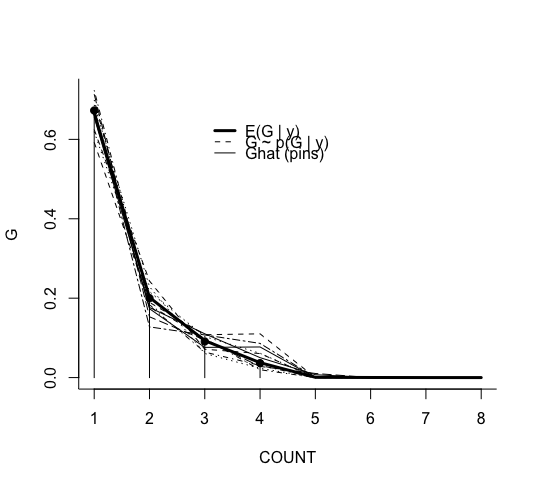
\includegraphics[width=0.58\textwidth]{./Poi.png}
  %\caption{\footnotesize gray: model (1) , black: model (2) , dashed line: observed value}
\end{figure}
\end{itemize}}

\section{Properties}
\subsection{}

\frame{\frametitle{Large Weak Support}
\begin{itemize}
  \item Under mild conditions, any distribution with the same support as $G_0$ can be well approximated weakly by a DP random probability measure
  \item Let $supp(Q)\subset supp(G_0 )$. For any finite number of measurable sets $A_1 ,\cdots,A_k $ and $\epsilon>0$, $$\pi\{|G(A_i )-Q(A_i )|<\epsilon,\ \text{for}\ i=1,\cdots,k\}>0$$ 
\end{itemize}}

\frame{\frametitle{Ferguson's Definition}
\begin{itemize}
  \item Random Variable $G(A)$ for any $A\subset\Theta$
  $$G(A)\sim\text{Beta}\left(MG_0 (A),M(1-G_0 (A))\right)$$
  $$E[G(A)]=G_0 (A),\ \ \ \ \ Var[G(A)]=\frac{G_0 (A)(1-G_0 (A))}{M+1}$$
  \item[-] $G_0$ : expected shape of $G$
  \item[-] $M$ : controls the variability of the realizations around $G_0$
  \item[-] $E(w_h )=\frac{1}{M+1}\left(\frac{M}{M+1}\right)^{h-1}\ \ \ \because v_h \stackrel{iid}{\sim}\text{Beta}(1,M)$ 
\end{itemize}}

\frame{\frametitle{Conjugacy}
\begin{itemize}
  \item $\theta_1 ,\cdots,\theta_n$ iid
  \item $\theta_i |G\sim G$ and $G\sim DP(M,G_0 )$
  \item Posterior
    $$\Rightarrow G| \theta_1 ,\cdots,\theta_n \sim \text{DP}\left(M+n,\frac{MG_0 +\sum \delta_{\theta_i}}{M+n}\right)$$
  \item Posterior Mean
  $$E(G|\theta_1 ,\cdots,\theta_n )=\frac{M}{M+n}G_0 + \frac{n}{M+n}\frac{\sum_{i=1}^{n}\delta_{\theta_i}}{n}$$
  \item Consistency
  \begin{itemize}
    \item[] since empirical cdf is consistent if iid, for some true distribution $G_T$, as $n\rightarrow\infty,\ G(A)|\theta_1 ,\cdots,\theta_n \stackrel{p}{\rightarrow}G_T (A)$ for any measurable set $A$
  \end{itemize}
\end{itemize}}

\frame{\frametitle{Simulation (Consistency)}
\begin{itemize}
  \item[-] true $G\sim N(2,2^2 )$
  \item[-] baseline $G_0 \sim N(0,1)$
  \item[-] $M=5$
\end{itemize}
\begin{figure}
  \centering
    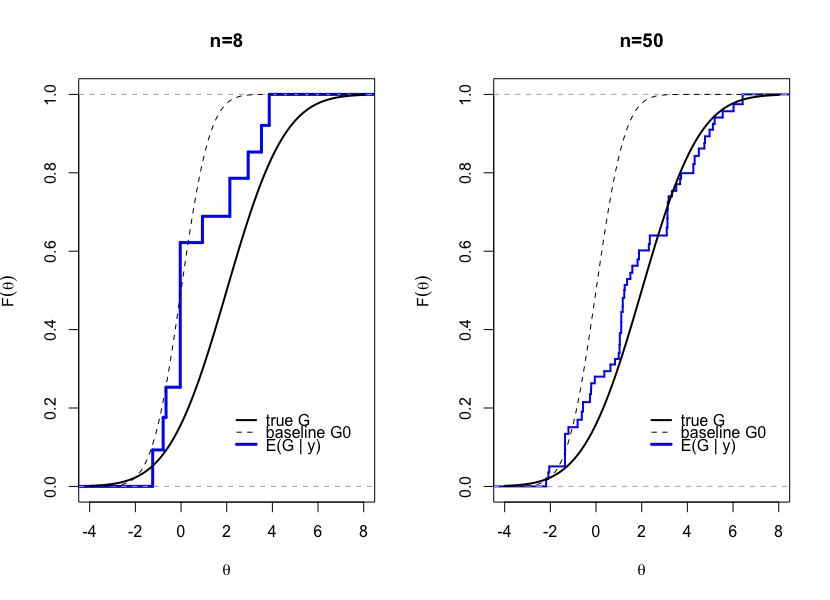
\includegraphics[width=0.68\textwidth]{./consistency.png}
  %\caption{\footnotesize gray: model (1) , black: model (2) , dashed line: observed value}
\end{figure}}

%\frame{\frametitle{Conditioning Property}
%\begin{itemize}
%  \item[-] $A$ is a measurable set with $G_0 (A)>0$ (thus, $G(A)>0$)
%  \item[-] Then, $G|_A (B)=G(B|A)=G(A\cap B)/G(A)\sim DP(M, G_0 |_A )$
%  \item[-] $G|_A (B)$ is independent of $G(A)$ 
%\end{itemize}}

\section{DPM}
\subsection{}

\frame{\frametitle{Dirichlet Process Mixtures}
\begin{itemize}
\item Motivation
\begin{itemize}
  \item[-] Discrete nature of DP
  \item[-] However, unknown distribution may be \textbf{continuous}
  \item[-] For some hierarchical models, DP prior may lead to inconsistent estimator when the true distribution is continuous.
\end{itemize}
\item Mitigation
\begin{itemize}
  \item[-] Add a convolution with a continuous kernel to $G$
\end{itemize}
\item DPM
$$y_1 ,\cdots,y_n \sim F(y_i )=\int P(y_i |\theta)\,G(d\theta),\quad G\sim \text{DP}(M,G_0 )$$
where $p(y_i |\theta)$ is a parametric distribution indexed by a finite dimensional parameter $\theta$.
\end{itemize}}

\frame{\frametitle{Stick-Breaking Construction}
$$y_i |(w_h ),(\tilde{\theta}_h )\sim \sum_{h=1}^{\infty}w_h P(y_i |\tilde{\theta}_h)=F(y_i )$$
$$\text{where}\; w_h = v_h \prod_{\ell<h} (1-v_{\ell}),\; v_h \sim \text{Beta}(1,M),\; \tilde{\theta}_h \sim G_0$$
\begin{itemize}
  \item[-] \textbf{countable} mixtures with an \textbf{infinite} number of components 
  \item[-] support on a large classes of distributions
\end{itemize}}

\frame{\frametitle{Clustering}
DPM induces clustering among the observations, with $M$ controlling the a priori expected number clusters in the sample.
  \begin{itemize}
    \item[-] $M\rightarrow0$: model reduces to a single component mixture (fully parametric model)
    $$y_i \stackrel{iid}{\sim}p(y|\theta),\quad \theta\sim G_0$$
    \item[-] $M\rightarrow\infty$: each observation assigned its own singleton cluster
    $$y_i \stackrel{iid}{\sim}\,\int p(y_i |\theta)G_0 (d\theta)$$
  \end{itemize}}

\frame{\frametitle{Hierarchical Model}
\begin{itemize}
  \item latent random effects $\theta_i$
  $$y_i |\theta_i \sim p(y_i |\theta_i ),\quad \theta_i |G \sim G,\quad G\sim \text{DP}(M,G_0 )$$
  \item highlighting the nature of clusters generated by ties among the $\theta_i$ 
  $$y_i |\theta_i \sim p(y_i |\theta_i ),\quad (\theta_1 ,\cdots,\theta_n )\sim p(\theta_1 ,\cdots,\theta_n )$$
\end{itemize}}

\frame{\frametitle{Cluster Indicator variable}
\begin{itemize}
  \item cluster indicator variables $(s_i )$ s.t. $\theta_i =\theta_{s_i}^*$
  $$y_i |s_i ,(\theta_j^* )\sim p(y_i |\theta_{s_i}^* ),\quad \theta_j^* \sim G_0 ,$$
  $$p(s_1 ,\cdots,s_n )=\frac{\Gamma(M)}{\Gamma(M+n)}M^k \prod_{j=1}^{k}\Gamma(n_j )$$
  where $k$: number of distinct values among $s_1 ,\cdots,s_n$ and $n_j =\sum_i I(s_i =j)$
  \begin{itemize}
    \item[-] prior distribution on all possible partitions of the data into at most $n$ groups
    \item[-] for any finite sample size $n$, at most $n$ distinct $\tilde{\theta}$ are sampled as $\theta_j^*$
  \end{itemize}
\end{itemize}}

\frame{\frametitle{Posterior Simulation for DPM Models}
$$y_i |\theta_i \sim p(y_i |\theta_i ),\quad \theta_i |G \sim G(\theta_i ),\quad G\sim \text{DP}(M,G_0 )$$
\begin{itemize}
  \item[-] kernel $p(y_i |\theta_i )$
  \item[-] unknown mixing measure $G\sim \text{DP}$ prior
\end{itemize}}

\frame{\frametitle{Collapsed Gibbs Samplers (Conjugate models)}
\begin{itemize}
  \item Species Sampling Model
  $$\theta_n |\theta_{n-1},\cdots,\theta_1 \sim \sum_{j=1}^{k_n -1}\frac{n_{n-1,j}}{M+n-1}\delta_{\theta_j^*}+\frac{M}{M+n-1}G_0$$
  where $n_{n-1,j}$: number of $\theta_i$ equal to $\theta_j^*$
  \begin{itemize}
    \item[-] \textbf{exchangeable}: full conditional prior distribution for any $\theta_i$ given $\theta_{-i}$
  \end{itemize}
\end{itemize}}

\frame{\frametitle{Full Conditional Posterior Distribution for $\theta_i$}
\begin{eqnarray*}
\theta_i |\theta_{-i},y &\propto& \sum_{j=1}^{k^-}n_j^- p(y_i |\theta_j^{*-})\delta_{\theta_j^{*-}}+M p(y_i |\theta_i )G_0 (\theta_i )\\
&=& \sum_{j=1}^{k^-}\{n_j^- p(y_i |\theta_j^{*-})\}\delta_{\theta_j^{*-}}+\\
&\,&\qquad \left\{M \int p(y_i |\theta_i )\, dG_0 (\theta_i )\right\}p(\theta_i |y_i ,G_0 )
\end{eqnarray*}
where $^-$: the appropriate quantity with $\theta_i$ excluded.
\begin{itemize}
  \item[-] $p(\theta_i |y_i ,G_0 )=\frac{p(y_i |\theta_i )\, dG_0 (\theta_i )}{\int p(y_i |\theta_i )\, dG_0 (\theta_i )}$: posterior on $\theta_i$ in a singleton cluster
  \item[-] $\int p(y_i |\theta_i )\, dG_0 (\theta_i )$: prior marginal distribution for $y_i$ under $G_0$
\end{itemize}}

\frame{\frametitle{Gibbs Sampler for $\theta_i$}
\begin{itemize}
  \item sample $\theta_i$ equal to one of the unique $\theta_j^*$'s with probability $\propto \; n_j^- p(y_i |\theta_j^* ) = n_{j}^{-}\int p\left(y_{i}|\theta_{i}^{*}\right)\,d\delta_{\theta_{j}^{*}}\left(\theta_{i}^{*}\right)$
  \item[] or
  \item sample from the posterior distribution based solely on $y_i$ with probability $\propto\; M\int p(y_i |\theta_i )\, dG_0 (\theta_i )$
  \item[]
  \item when the mixture components are well separated, slow mixing
  \item faster mixing by including an additional transition probability
  \item more efficient sampler by first sampling indicators from $p(s_i |s^- ,y)$ sequentially and then sampling each $\theta_j^*$ from $p(\theta_j^* |y,s)$
\end{itemize}}

\frame{\frametitle{$p(s_i |s^- ,y)$}
\begin{itemize}
\item hierarchical model
$$p(s_i =j|s^- ,\theta^{*-},y)\propto\left\{\begin{array}{ll}n_j^- p(y_i |\theta_j^{*-})&j=1,\cdots,k^-\\
M\int p(y_i |\theta_i )\, dG_0 (\theta_i )&j=k^- +1 \end{array}\right.$$
and
$$p(\theta_i |s_i =j, s^- ,\theta^{*-},y)=\left\{\begin{array}{ll}\delta_{\theta_j^{*-}} & j=1,\cdots,k^-\\
p(\theta_i | y_i ,G_0 ) & j=k^- +1 \end{array}\right.$$
\end{itemize}}

\frame{\frametitle{$p(s_i |s^- ,y)$}
\begin{itemize}
  \item[-] $\mathbf{y}_j^{*-}=(y_{\ell};\,s_{\ell}=j \,\text{and}\, \ell\neq i)$: obs in the $j$th cluster w/o $y_i$
  \item[-] Remove $\theta_j^{*-}$ from the conditioning set by integrating with respect to $p(\theta_j^{*-}|s^- ,y)=p(\theta_j^{*-}|y_j^{*-})$
  $$p(s_i =j|s^- ,y)\propto\left\{\begin{array}{ll}n_j^- \int p(y_i |\theta_j^{*-} )\, dp(\theta_j^{*-}|y_j^{*-} ) & j\leq k^- \\
  M\int p(y_i |\theta_i )\, dG(\theta_i ) & j=k^- +1
  \end{array}\right.$$
  \item[-] Full conditional posterior for $\theta_j^*$
  $$p(\theta_j^* |s,y)\propto G_0 (\theta_j^* )\prod_{\{i:s_i =j\}}p(y_i |\theta_j^* )$$
  \item[-] When $G_0 (\theta)$ is conjugate to $p(y_i |\theta)$, all of $\int p(y_i |\theta_j^{*-})\,dp(\theta_j^{*-}|y_j^{*-}),\; \int p(y_i |\theta_i )\, dG_0 ,\; p(\theta_j^* |s,y)$ are usually available in closed form and implementation of the algorithm is straightforward.
\end{itemize}}

\end{document}
%\frame{\frametitle{Production Partition Model (PPM)}
%\begin{itemize}
%  \item Cohesion Function $$c(S_j )=M(n_j -1)$$
%  \item Special case of the Polya Tree with $\alpha_{\epsilon}=\alpha_{\epsilon0}+\alpha_{\epsilon1}$
%\end{itemize}}

%\frame{\frametitle{Neutral to the Right Process}
%\begin{itemize}%

%\end{itemize}}

\frame{\frametitle{}
\begin{itemize}

\end{itemize}}

\frame{\frametitle{}
\begin{itemize}

\end{itemize}}

\frame{\frametitle{}
\begin{itemize}

\end{itemize}}
  
\end{document}